%%%%%%%%%%%%%%%%%%%%%%%%%%  phdsymp_sample2e.tex %%%%%%%%%%%%%%%%%%%%%%%%%%%%%%
%% changes for phdsymp.cls marked with !PN
%% except all occ. of phdsymp.sty changed phdsymp.cls
%%%%%%%%%%                                                       %%%%%%%%%%%%%
%%%%%%%%%%    More information: see the header of phdsymp.cls   %%%%%%%%%%%%%
%%%%%%%%%%                                                       %%%%%%%%%%%%%
%%%%%%%%%%%%%%%%%%%%%%%%%%%%%%%%%%%%%%%%%%%%%%%%%%%%%%%%%%%%%%%%%%%%%%%%%%%%%%%


%\documentclass[10pt]{phdsymp} %!PN
\documentclass[twocolumn]{phdsymp} %!PN
%\documentclass[12pt,draft]{phdsymp} %!PN
%\documentstyle[twocolumn]{phdsymp}
%\documentstyle[12pt,twoside,draft]{phdsymp}
%\documentstyle[9pt,twocolumn,technote,twoside]{phdsymp}

\usepackage[english]{babel}       % Voor nederlandstalige hyphenatie (woordsplitsing)

\usepackage{graphicx}                   % Om figuren te kunnen verwerk
\usepackage{graphics}			% Om figuren te verwerken.
\graphicspath{{figuren/}}               % De plaats waar latex zijn figuren gaat halen.

\usepackage{cleveref}
\usepackage{times}

\hyphenation{si-mu-la-ted re-a-lis-tic packets really in-clu-ding}

\def\BibTeX{{\rm B\kern-.05em{\sc i\kern-.025em b}\kern-.08em
    T\kern-.1667em\lower.7ex\hbox{E}\kern-.125emX}}

\newtheorem{theorem}{Theorem}

\begin{document}

\title{Optimization of client-side intermodal \\route planning} %!PN

\author{Brecht Van de Vyvere}

\supervisor{Pieter Colpaert, Ruben Verborgh, Erik Mannens, Rik Van de Walle}

\maketitle

%   - context
%   - need
%   - task
%   - object
%   - findings
%   - conclusion
%   - perspectives
   
\begin{abstract}
Route planning of public transit is an active research domain. To calculate routes that meets the users requirements, an extensible and fast route planning system is needed. Linked Connections is a framework that solves route planning queries on the client. This paper introduces a speedup method to accelerate Linked Connections. This is done with the vision of Linked Data Fragments (LDFs). A new type of LDF makes extra filtering possible which leads to 38\% less data usage. The tested implementation executes local queries 37\% faster.
% There's still much space for improvement with long distance queries.
\end{abstract}

\begin{keywords}
Linked Connections, optimization, route planning, client-side, GTFS
\end{keywords}

\section{Introduction}
\PARstart{R}{oute} planning is at the beginning of an evolution, just like the Web did in the \textit{nineties}. On the one hand, you have commuters that want to know which vehicles take them from point A to B. On the other hand, you have public transit companies that provide services that calculate which route you can take. Since a few years, more and more companies share their time schedules in the uniform formats \textit{General Transit Feed Specification} (GTFS) and \textit{GTFS-RealTime} as Open Data. Data is getting available, but the dots need to be connected. Not only with other transit data from around the world, but also with all the data that the Web has to offer.

Nowadays, route planners are build with an Application Programming Interface (API). This works well for certain applications, but extending it with new features is limited.
Another limitation of an API is that the client can't control which information it wants to use and make smart decisions. This can be solved by using one of the core aspects of the Web: hypermedia. This means that clients are able to retrieve information by following links.
\\~\\
Now that certain necessities for route planning are explained, we will first discuss some related work. After that, we'll tell more about \textit{Linked Connections} and how it tries to solve above issues. Next, we introduce two optimization methods that will be evaluated thereafter. Finally, some concluding remarks will be made.

\section{Related work}
In the first two subsections we will discuss briefly what types of route planning algorithms are available. After that, we'll tell more about moving intelligence to the client and how it can be used for route planning.

\subsection{Dijkstra}
Route planning has been solved traditionally with Dijkstra algorithm \cite{raptor}. This means that public transit networks are modelled as a graph-based network and Dijkstra calculates the shortest path between a source node and every other node. Several optimization techniques have been introduced to achieve query times within milliseconds\cite{scalable-transfer-patterns}. These techniques often result in long pre-processing time and/or large space consumption.

\subsection{CSA}
\label{csa}
Since 2013, the Connection Scan Algorithm (CSA) \cite{csa} makes route planning a data problem, instead of a mathematical one. 
A connection $c$ represents a vehicle that departs in a certain departure stop $c_{depstop}$ and arrives in a certain arrival stop $c_{arrstop}$ without stopping. Also an indication of the departure time $c_{deptime}$ and arrival time $c_{arrtime}$ is contained within a connection. Connections can be retrieved out of e.g. a \textit{General Transit Feed Specification} (GTFS) feed. Like the name suggests, route planning queries can be solved by scanning a list of connections. The only restriction is that the connections have to be sorted by their departure time $c_{deptime}$. While scanning, a Minimum Spanning Tree (MST) is build holding connections that produce the fastest route from the departure stop at a certain departure time to every other stop. \textit{Earliest Arrival Time} (EAT) queries can easily be solved with this MST. Other query types can also be calculated with CSA, but are more complex. For example: \textit{profile} queries return multiple routes within a time interval. This research will focus on EAT queries.

\subsection{Linked Data Fragments}
Linked Data Fragments (LDFs, \cite{verborgh_ldow_2014}) is a vision that makes it possible to capture a certain part of a dataset. Every fragment type has a \textit{selector} function that selects the data that belongs to it. Also \textit{metadata} and \textit{hypermedia controls} define a fragment. It's purpose is to let clients efficiently execute queries on these datasources. By placing these types of fragments on an axis (\cref{LDF-asFinalAbstract}), different trade-offs between client and server can be discussed. This axis shows the amount of effort that needs to be done by data consumers and data publishers. One of the advantages of LDFs is the possibility to cache the documents. This enables servers to be low-cost.

\subsection{Linked Connections}
\label{lc}

Linked Connections (LC, \cite{colpaert_iswc_2015}) is a framework that enables clients to execute route planning queries on data sources. Servers are only responsible for publishing LDFs that contain connections (\cref{csa}), so called \textit{Linked Connections Fragments} (LCFs). A LCF is a type of LDF and contains connections from a subset of stops $S$ from a dataset. Hypermedia controls give clients the possibility to retrieve more information, e.g. where to find a next fragment or metadata about a stop.
You can see in \cref{LDF-asFinalAbstract} a LDF-axis representing LCFs. (1) represents the original implementation of LC. (2) and (3) are respectively the heuristic and speedup optimizations that will be futher discussed in \cref{optimization}. In next subsection, we explain how LC currently publishes its connections with \textit{basic LCFs} (BLCFs).

\begin{figure}[ht]
\begin{center}
	\includegraphics[width=.50\textwidth]{LDF-asFinalAbstract}
	\caption{\label{LDF-asFinalAbstract}Linked Data Fragments-axis for public transit route planning. On the left, you can see data dumps, e.g. GTFS files. On the right, you have web services that provide certain functionality to clients. Linked Connections tries to find new ways to plan routes by publishing transit data using different types of fragments.}
\end{center}
\end{figure}

\subsubsection{Basic Linked Connections Fragment}

A \textit{basic} LCF (BLCF) contains every connection $c$ that has a departure time between a certain time interval $F_{start}$ and $F_{end}$. For example, these time intervals can be fixed to every $X$ minutes or precalculated so every fragment has a similar size of connections. The subset of stops $S$ of a BLCF contains every stop of the dataset. \Cref{hypermediafragmenten} shows how BLCFs have a \textit{nextPage}-link to the next fragment and that connections are ordered by departure time.
A client can now download the fragment as data source and input the connections to CSA. Until a solution is found or certain conditions are reached, e.g. maximum query time, the client fetches next fragments.
Route planning with only BLCFs has already been implemented before this research, so we'll call this the \textit{original} method.

\begin{figure}[ht]
\begin{center}
	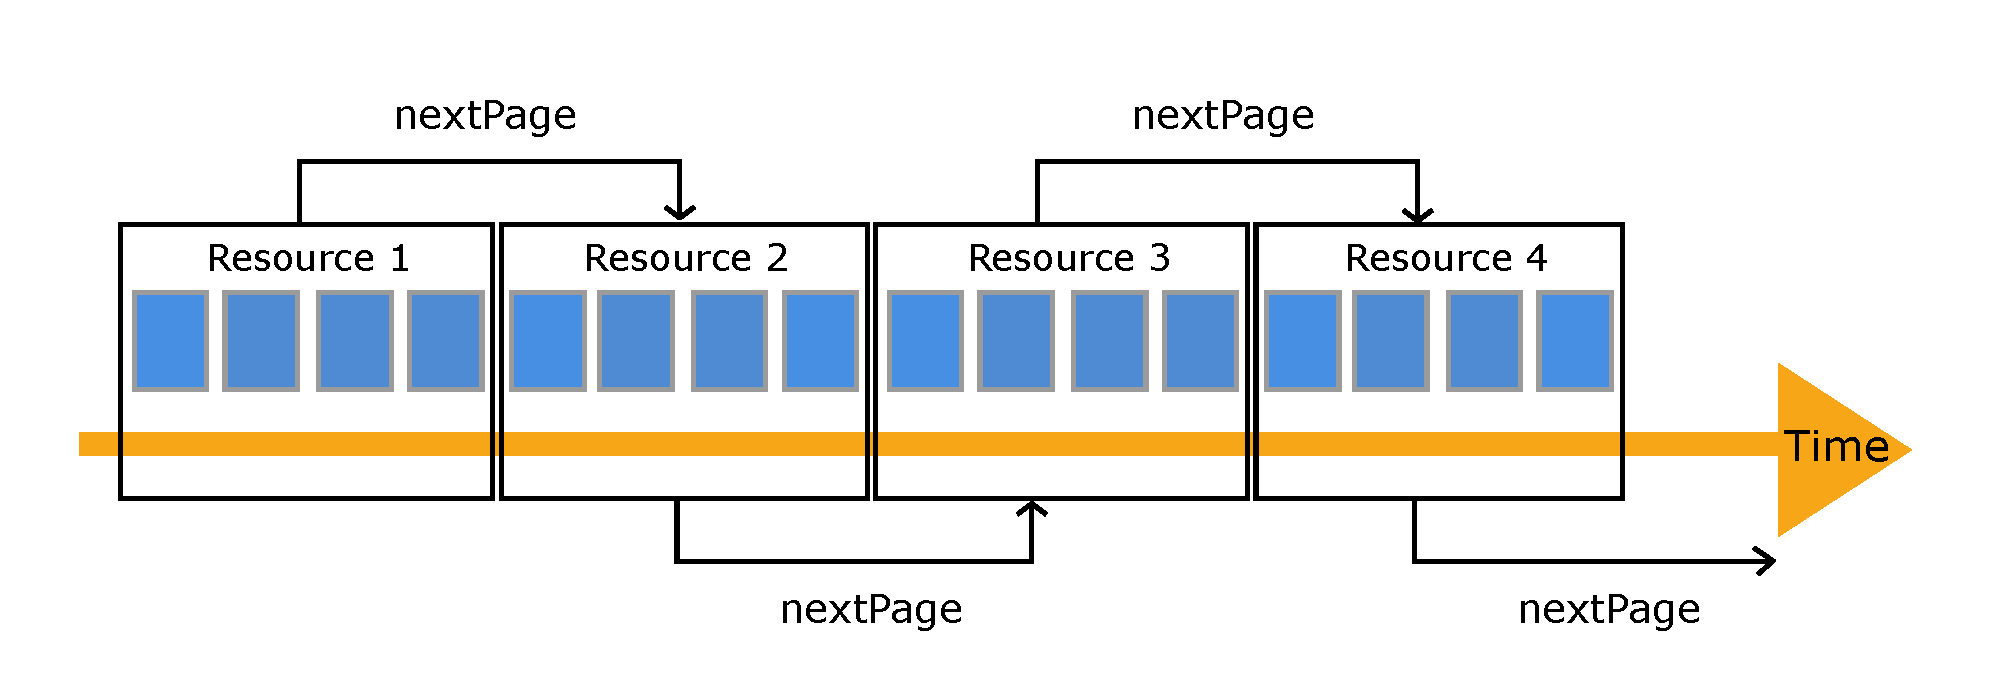
\includegraphics[width=.50\textwidth]{hypermediafragmenten}
	\caption{\label{hypermediafragmenten}A \textit{basic} LCF represents all connections between a certain time range.}
\end{center}
\end{figure}

This way of publishing makes a server very low-cost, because the amount of possible fragments is limited. Each fragment corresponds with one URL.
 \Cref{lc:aantalurisoorspronkelijk} shows the amount of URLs when all minutes of a day are spread by a fixed time interval $F$. If $F$ is equal to 10 minutes, then there would be 144 URLs. Most public transit companies are not always active (for example: after midnight), so the amount of non-empty fragments is practically lower.
\begin{equation} \label{lc:aantalurisoorspronkelijk}
24 * 60 / F
\end{equation}

This method causes the client to scan a lot of \textit{useless} connections. This means that the connection is not added to the Minimum Spanning Tree (MST) of CSA. BLCFs return connections from every stop of the dataset between that time period. E.g.: when you depart in Brussels, you're not interested in connections from Madrid at that moment.
To address this issue, we introduce a new type of LDF in \cref{nlcf}.

\section{Neighbour Linked Connections Fragment}
\label{nlcf}

In a \textit{neighbour} LCF, connections are returned depending relative to the $query_{deptime}$ and $query_{depstop}$. $S$ represents the $query_{depstop}$ and its neighbouring stops within a certain maximum amount of possible transfers $K_{max}$. A \textit{transfer} occurs when there is a change of vehicle. Futher, every stop $s$ of $S$ has its own time interval of connections that belong to the fragment.
By also providing information about the departure stop, a connection $c$ can be dropped if $c_{deptime} < R(query_{depstop}, c_{depstop})$. For the previous example: when departing from Brussels, connections that depart in Spain on the same moment won't be returned.
The use of a NLCF allows better filtering, especially in the beginning. Less connections need to be scanned so CSA can advance faster in time.

Public transit is not symmetrically: going from stop A to B can be different in the opposite direction. Following two features need to be pre-processed for every pair stops ($A$, $B$):
\begin{itemize}
\label{prefeatures}
\item The minimum amount of transfers $K(A, B)$.
\item The minimum amount of time $R(A, B)$. This has not the same meaning of the fastest route, but is equal to the sum of the edges of the shortest path from A to B in a graph (\cref{pre-processing}).
\end{itemize}

\subsection{Pre-processing}
\label{pre-processing}

Pre-processing of above features (\cref{prefeatures}) requires two additional steps.
\begin{enumerate}
\item Calculate $R(A,B)$ for every pair direct reachable stops $A$ and $B$. A stop is direct reachable if it can be reached with one trip ($K(A,B) = 0$). This information can be fetched by looping through the \textit{stop\_times.txt} file of a \textit{GTFS} feed or while generating connections.
\item Calculate $R(A,B)$ and $K(A,B)$ for every stop $A$ in the dataset to every indirect ($K(A,B)>0$) reachable stop $B$.
\end{enumerate}

\Cref{table:calcneighbours} shows the amount of pre-processing time to calculate $R(A,B)$ and $K(A,B)$ for every pair of stops $(A,B)$ of a dataset.
\begin{table}[htbp]
\centering
\begin{tabular}{ | c || c | c | }
  \hline
  Dataset & Amount of stops & Pre-processing time (min) \\ \hline
  NMBS\footnote{Belgian railway company} & 597 & 6,35 \\
  NS\footnote{Dutch railway company} & 2532 & 21,19 \\
\hline  
\end{tabular}
\caption{Time to calculate indirect reachable stops for every stop in a \textit{GTFS} feed.}
\label{table:calcneighbours}
\end{table}

\section{Optimization}
\label{optimization}

This research has tested two optimizations. First, we introduce a method (\cref{heuristic}) that uses a heuristic to determine a next NLCF.  The second optimization (\cref{speedup}) uses the benefits of the heuristic method to speedup the original method.

\subsection{Heuristic}
\label{heuristic}

The heuristic method ((2) on \cref{LDF-asFinalAbstract}) solves queries by only using NLCFs. Every stop $s$ of the NLCF uses the same time range $T$ (\cref{neighbourconnections}). 
$T$ and $K_{max}$ can be changed dynamically on the server.
The optimal route is found if every connection $c$ of that route has following properties:
\begin{itemize}
\item $ ( query_{deptime} + R(query_{depstop}, c_{depstop}) ) <= c_{deptime} < c_{depstop} + T$: $c$ departs within the time range of stop $c_{depstop}$
\item $c_{depstop} \in S$ with $S$ determined by a maximum amount of allowed transfers $K_{max}$
\end{itemize}

\begin{figure}[ht]
\begin{center}
	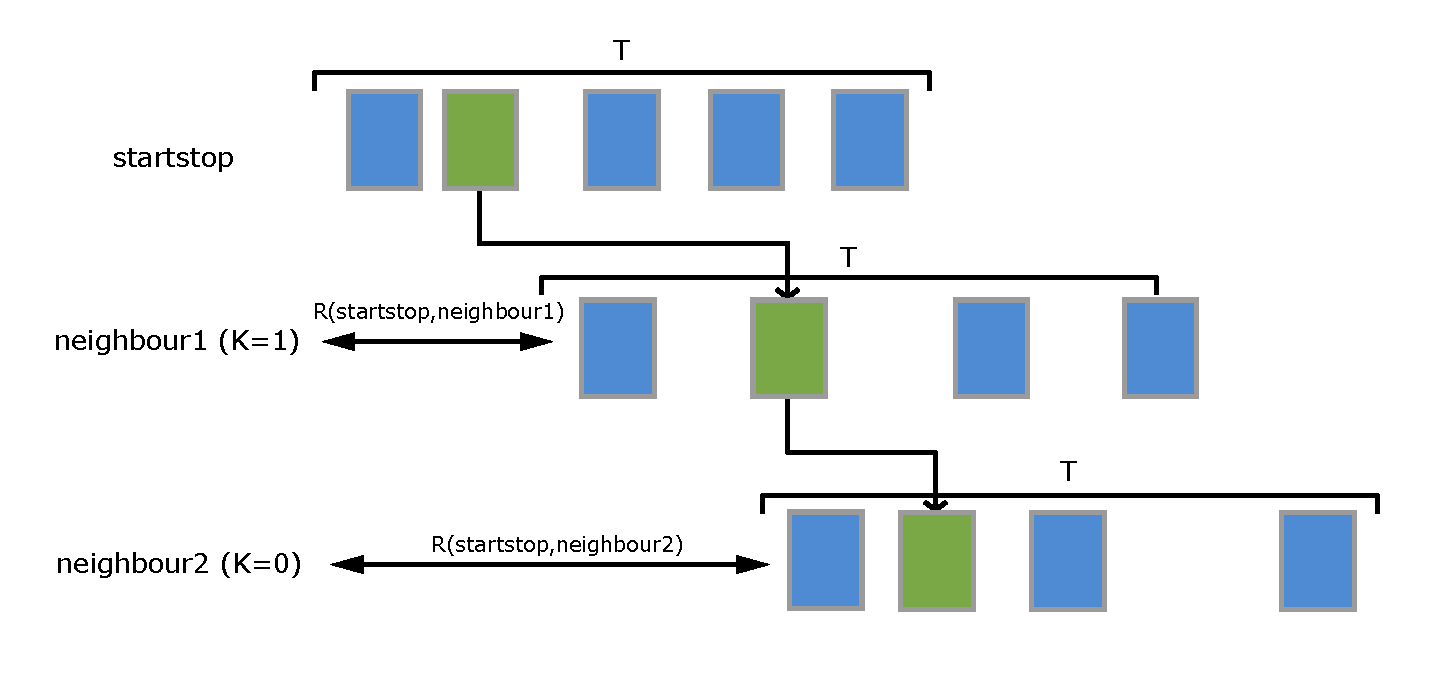
\includegraphics[width=.50\textwidth]{Burenconnecties}
	\caption{\label{neighbourconnections}Overview of connections that are returned with a Neighbour LC Fragment for the heuristic optimization. Note that the amount of stops is limited by a maximum amount of allowed transfers $K_{max}$.}
\end{center}
\end{figure}

If the fastest route isn't found then a next NLCF needs to be fetched by the client. The heuristic method does this by holding a priority queue of reached stops. Every \textit{usefull} connection $c$ is analysed and gets a priority defined by \cref{priorityfunction}:
\begin{equation} \label{priorityfunction}
priority(c) = \alpha * c_{v} + \beta * c_{arrstop}[importance] + \gamma * \cos(\theta)
\end{equation}

Parameters that are used:
\begin{itemize}
\item \textit{Velocity} $c_{v}$ is distance over time of the connection.
\item \textit{Importance} of a stop is indicated by the amount of direct reachable stops.
\item \textit{Cosine simularity} shows if $c$ is going in the right direction. $\theta$ is the degree between the connection $c$ vector and the vector between $query_{depstop}$ and $query_{arrstop}$.
\end{itemize}

Each parameter is divided by the maximum value that occurs in the fragment so its value is normalized.$\alpha$, $\beta$ and $\gamma$ are weight factors that can be altered to give certain parameters more impact.

The heuristic method results in a suboptimal solution if a next stop is chosen that doesn't belong to the optimal route and the destination gets reached. It depends of the chosen stop how many minutes longer the route takes. The results (\cref{results}) will show that most queries can be solved with the first NLCF.
The next method (\cref{speedup}) combines the use of this first NLCF together with BLCFs to guarantee the fastest route.

\subsection{Speedup}
\label{speedup}

The speedup method accelerates the original method by using one NLCF initially. This NLCF is split in multiple pages with hypermedia links holding them together (\cref{NLCFpaged}). This way, the size of pages remain compact. The NLCF uses one global time interval $T$ for all the stops.

\begin{figure}[ht]
\begin{center}
	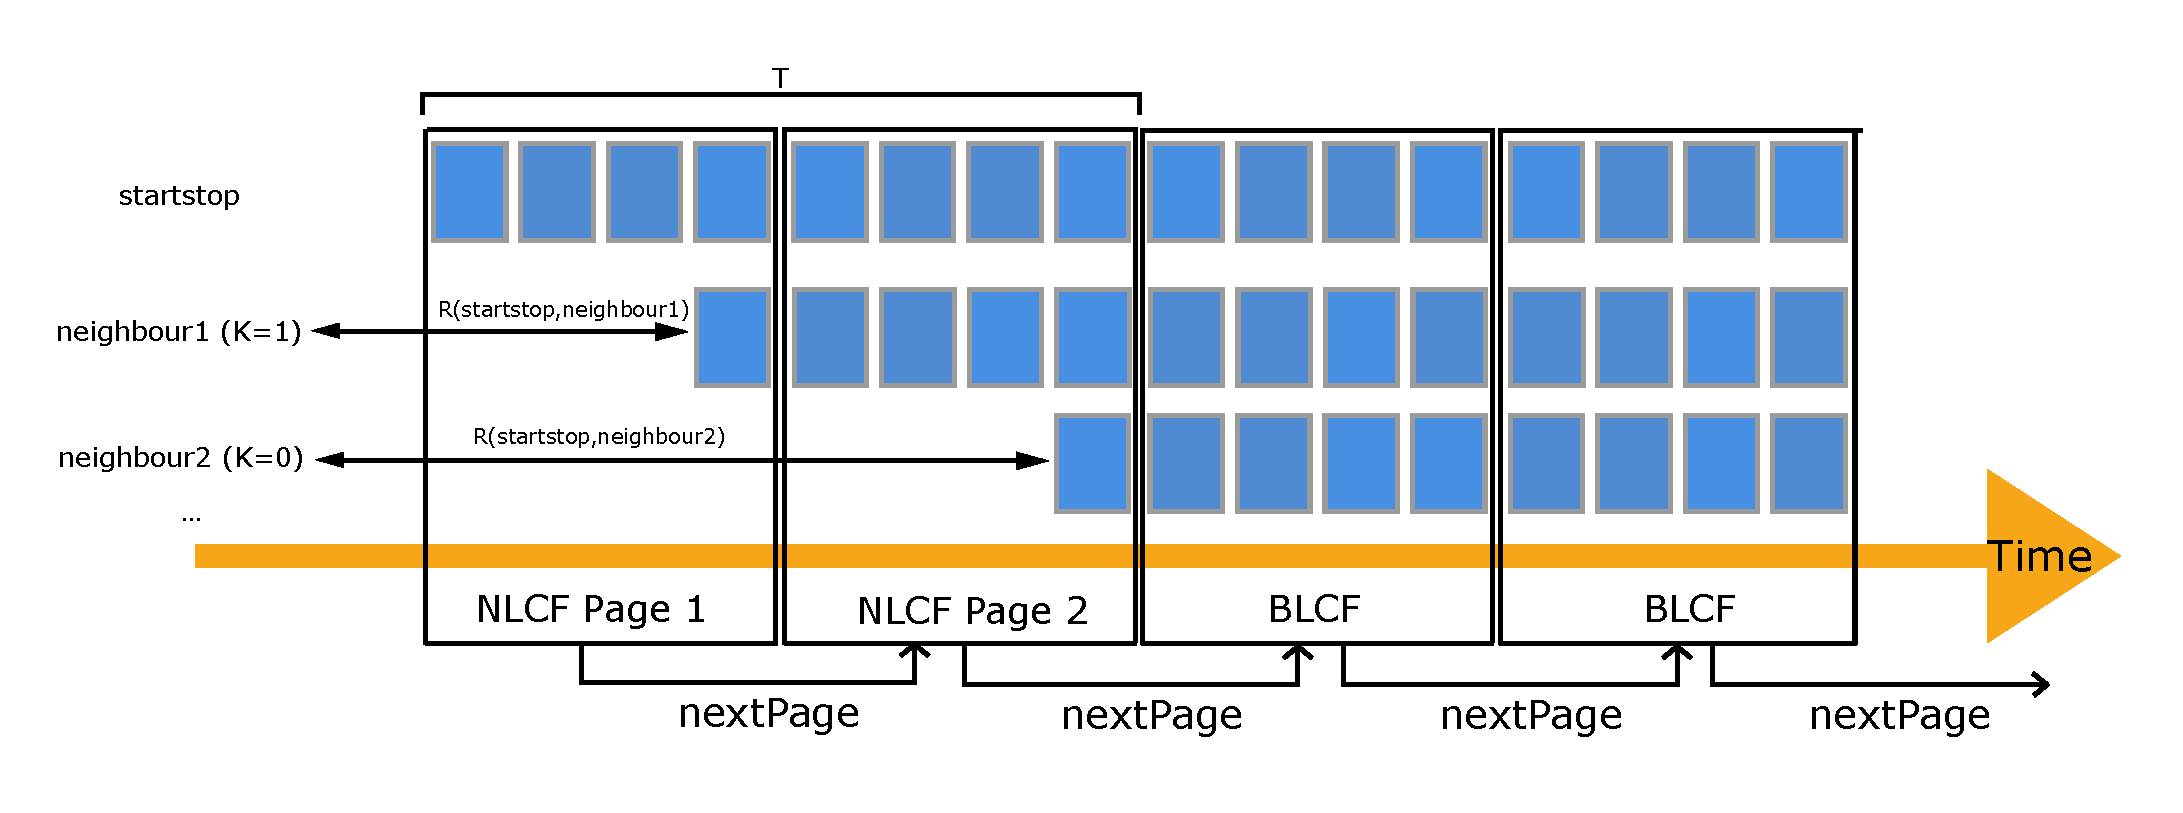
\includegraphics[width=.50\textwidth]{NLCFpaged}
	\caption{\label{NLCFpaged}Overview of the speedup technique. First a NLCF is used to filter connections by the departure time and departure stop of the query. After a certain time period $T$, basic LCFs are used.}
\end{center}
\end{figure}

To guarantee that the fastest route can be found, all stops of the dataset need to be included ($K_{max}$ represents every stop) in the NLCF. After $T$, hypermedia \textit{nextPage}-links refer back to BLCFs. The size of $T$ depends off the dataset. For the NMBS, the Belgian railway company, most stops can be reached within 120 - 150 minutes. After that time, NLCF pages are similar to BLCFs.
This speedup method is the most centered line (3) on the LDF-axis (\cref{LDF-asFinalAbstract}) because it requires three HTTP parameters: the departure time, departure stop and page number. This causes less caching possibilities for the server thus higher server effort.

\section{Evaluation}
\label{evaluation}

\textit{Earliest Arrival Time} $queries$ have been tested. Such queries exist out of three components: the stop where the route starts $query_{depstop}$, the destination $query_{arrstop}$ and a time of departure $query_{deptime}$. The result is the fastest route between those two stops starting from the departure time. The amount of transfers is not considerated as criteria.
A web application has been developed to compare all three methods: the original, heuristic and speedup. 900 queries are generated out of the NMBS GTFS feed, which contains 644 stops and 127116 connections for one day.  All tests have been run on a Macbook Pro 2015 with 8 GB RAM and Intel Core i5 2,7 Ghz CPU. 
There are still software issues, such as stations that are hard to reach, which causes the client to stop searching. The results are representative for local, in Belgium located, stations. 
The time interval of a basic LCF is limited to every 20 minutes, representing 1100 connections on average. Neighbour LCFs of the heuristic method use a time interval of 100 minutes. The NLCF of the speedup method uses a time interval of 120 minutes split in pages of 30 minutes.

\section{Results}
\label{results}

\subsection{Speed}

\Cref{timedistancewithcaching} shows the time to plan a route according to the distance of the route in bird flight. The original method (in blue) and speedup method (in red) both grow linear with the distance. It is clear that the speedup method accelerates the original method with seconds, because less connections need to be scanned. On average, the speedup method makes querying 37\% faster then the original method.
The heuristic method in yellow follows a different pattern. Almost all query times are located on a horizontal line of 2 seconds. This means that these queries are all solved with the first NLCF. Only a few queries are solved with multiple NLCFs. Note that 22\% of the results of the heuristic method are not displayed due to a suboptimal solution. The routes that are optimal are 57\% faster then the original method.
\begin{figure}[ht]
\begin{center}
	
\includegraphics[width=.50\textwidth]{timedistancewithcaching}
	\caption{\label{timedistancewithcaching}Time to calculate queries according to the distance of the route.}
\end{center}
\end{figure}

\subsection{Data usage}

Another important aspect is data usage. The use of NLCFs makes better filtering possible. You can see in \cref{datausagedistance} how much data consumption has been lowered with the optimization methods. Speedup has clearly the advantage. It uses less data then the heuristic method, because the NLCF is paged. The surplus of connections that are downloaded is smaller with pages then downloading the whole NLCF. The speedup method reduces the amount of data with 38\% on average.
The heuristic method also uses less data then the original method, because connections are better filtered by the server.
Less data usage can also be an advantage in a setup where internet connectivity is sparse.

\begin{figure}[ht]
\begin{center}
	
\includegraphics[width=.50\textwidth]{datausagedistance}
	\caption{\label{datausagedistance}Overview of data consumption. An extra filter by departure stop enables the server to drop connections that are useless and don't need to be sent.}
\end{center}
\end{figure}

\Cref{table:summary} gives a summary of the results regarding speed, data consumption and usefull connnections.
\begin{table}[htbp]
\centering
\begin{tabular}{ | l || c | c | c |}
\hline
  & Basic & Speedup & Heuristic  \\ \hline
  Speed (s) & 4.54 & 2.87 & 1.96 \\
  Data usage (MB) & 2.69 & 1.68 & 1.97 \\
  Usefull connections (\%) & 0.026 & 0.047 & 0.064 \\
  Optimal & yes & yes & no \\
\hline  
\end{tabular}
\caption{}
\label{table:summary}
\end{table}

\section{Conclusion}
In this paper, we have implemented three methods to solve route planning queries with Linked Connections. As base line, we have tested how fast route planning works with only \textit{basic} Linked Connections Fragments. We introduced two different methods that use an extra filter based on the departure stop and departure time of the query. Pre-processing time is limited to minutes. The heuristic method is the fastest, but only returns the optimal result for 78\% of the tested queries. The speedup method makes querying 37\% faster then the original method while guaranteeing the optimal solution. Also bandwidth is saved by 38\%.

\nocite{*}
\bibliographystyle{phdsymp}
%%%%%\bibliography{bib-file}  % commented if *.bbl file included, as
%%%%%see below


%%%%%%%%%%%%%%%%% BIBLIOGRAPHY IN THE LaTeX file !!!!! %%%%%%%%%%%%%%%%%%%%%%%%
%% This is nothing else than the phdsymp_sample2e.bbl file that you would%%
%% obtain with BibTeX: you do not need to send around the *.bbl file        
%%
%%---------------------------------------------------------------------------%%
%
\begin{thebibliography}{1}

\bibitem{raptor}
Daniel Delling and Thomas Pajor and Renato F. Werneck,
\newblock {\em Round-Based Public Transit Routing },
\newblock { Transportation Science, pages 591-604, 2015}

\bibitem{scalable-transfer-patterns}
Hannah Bast and Matthias Hertel and Sabine Storandt,
\newblock {\em Scalable Transfer Patterns},
\newblock { 2016 Proceedings of the Eighteenth Workshop on Algorithm Engineering and Experiments (ALENEX) }

\bibitem{csa}
Dibbelt, Julian and Pajor, Thomas and Strasser, Ben and Wagner, Dorothea,
\newblock {\em Intriguingly Simple and Fast Transit Routing},
\newblock {Experimental Algorithms, pages 43-54,. Springer, 2013. }

\bibitem{colpaert_iswc_2015}
Colpaert, Pieter and Llaves, Alejandro and Verborgh, Ruben and Corcho, Oscar and Mannens, Erik and Van de Walle, Rik,
\newblock {\em Intermodal public transit routing using {Linked Connections}},
\newblock {Proceedings of the 14th International Semantic Web Conference: Posters and Demos, oct. 2015}

\bibitem{verborgh_ldow_2014}
Verborgh, Ruben and Vander Sande, Miel and Colpaert, Pieter and Coppens, Sam and Mannens, Erik and Van de Walle, Rik,
\newblock {\em Web-Scale Querying through {Linked Data Fragments} },
\newblock {Proceedings of the 7th Workshop on Linked Data on the Web, apr. 2014}


\bibitem{gtfs-ref}
\newblock {\em GTFS reference},
\newblock https://developers.google.com/transit/gtfs/reference

\end{thebibliography}
%
%%---------------------------------------------------------------------------%%

\end{document}

%%%%%%%%%%%%%%%%%%%%%  End of phdsymp_sample2e.tex  %%%%%%%%%%%%%%%%%%%%%%%%%%%
